\documentclass[crop, tikz]{standalone}

\usepackage[utf8]{inputenc}
% 'crop' is the default for v1.0, before it was 'preview'
%\usetikzlibrary{...}% tikz package already loaded by 'tikz' option

\usetikzlibrary{arrows}
\usetikzlibrary{decorations.markings}
\usetikzlibrary{patterns}
\usetikzlibrary{calc}

\begin{document}

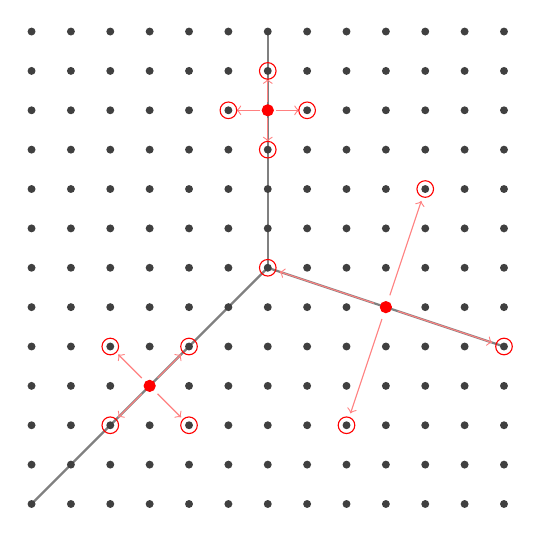
\begin{tikzpicture}[]

	% skeleton node placement
	\coordinate (v0) at (0,0);
	\coordinate (v1) at (-3,-3);
	\coordinate (v2) at (0,3);
	\coordinate (v3) at (3,-1);
	% skeleton colour scheme
	\def\options{black!50!white}

	% draw the skeleton
	\draw[thick, \options] (v0) -- (v1);
	\draw[thick, \options] (v0) -- (v2);
	\draw[thick, \options] (v0) -- (v3);
	\filldraw[fill=\options] (v0) circle (1pt);

	% draw node placement
	\foreach \i in {-3,-2.5,...,3} {
		\foreach \j in {-3,-2.5,...,3} {
			\filldraw[thick, black!75!white] (\i,\j) circle (1pt);
		} 
	}

	% nearest neighbours for straight edge
	\coordinate (straightNode) at ($(v0)!0.6666!(v2)$);
	\filldraw[red] (straightNode) circle (2pt);
	% arrows for connections
	\draw[red!50!white, ->] ($(straightNode)-(0,0.1)$) -- ($(straightNode)-(0,0.4)$);
	\draw[red!50!white, ->] ($(straightNode)+(0,0.1)$) -- ($(straightNode)+(0,0.4)$);
	\draw[red!50!white, ->] ($(straightNode)-(0.1,0)$) -- ($(straightNode)-(0.4,0)$);
	\draw[red!50!white, ->] ($(straightNode)+(0.1,0)$) -- ($(straightNode)+(0.4,0)$);
	% circle nodes that are involved
	\draw[red] ($(straightNode)-(0,0.5)$) circle (3pt);
	\draw[red] ($(straightNode)+(0,0.5)$) circle (3pt);
	\draw[red] ($(straightNode)-(0.5,0)$) circle (3pt);
	\draw[red] ($(straightNode)+(0.5,0)$) circle (3pt);


	% nearest neighbours for 1:1 diagonal edge
	\coordinate (diag11) at ($(v0)!0.5!(v1)$);
	\filldraw[red] (diag11) circle (2pt);
	% arrows for connections
	\draw[red!50!white, ->] ($(diag11)+(0.1,0.1)$) -- ($(diag11)+(0.4,0.4)$);
	\draw[red!50!white, ->] ($(diag11)+(-0.1,0.1)$) -- ($(diag11)+(-0.4,0.4)$);
	\draw[red!50!white, ->] ($(diag11)+(0.1,-0.1)$) -- ($(diag11)+(0.4,-0.4)$);
	\draw[red!50!white, ->] ($(diag11)+(-0.1,-0.1)$) -- ($(diag11)+(-0.4,-0.4)$);
	%circle nodes that are involved
	\draw[red] ($(diag11)+(0.5,0.5)$) circle (3pt);
	\draw[red] ($(diag11)+(-0.5,0.5)$) circle (3pt);
	\draw[red] ($(diag11)+(0.5,-0.5)$) circle (3pt);
	\draw[red] ($(diag11)+(-0.5,-0.5)$) circle (3pt);

	% lack of "nearest" neighbours for 3:-1 edge
	\coordinate (diag31) at ($(v0)!0.5!(v3)$);
	\filldraw[red] (diag31) circle (2pt);
	% arrows for connections
	\draw[red!50!white, ->] ($(diag31)+0.05*(3,-1)$) -- ($(diag31)+0.45*(3,-1)$);
	\draw[red!50!white, ->] ($(diag31)-0.05*(3,-1)$) -- ($(diag31)-0.45*(3,-1)$);
	\draw[red!50!white, ->] ($(diag31)+0.05*(1,3)$) -- ($(diag31)+0.45*(1,3)$);
	\draw[red!50!white, ->] ($(diag31)-0.05*(1,3)$) -- ($(diag31)-0.45*(1,3)$);
	%circle nodes that are involved
	\draw[red] ($(diag31)+(1.5,-0.5)$) circle (3pt);
	\draw[red] ($(diag31)-(1.5,-0.5)$) circle (3pt);
	\draw[red] ($(diag31)+(0.5,1.5)$) circle (3pt);
	\draw[red] ($(diag31)-(0.5,1.5)$) circle (3pt);

\end{tikzpicture}

\end{document}